\documentclass[11pt]{scrartcl}
\usepackage{tkz-graph}


\begin{document}
\begin{center}
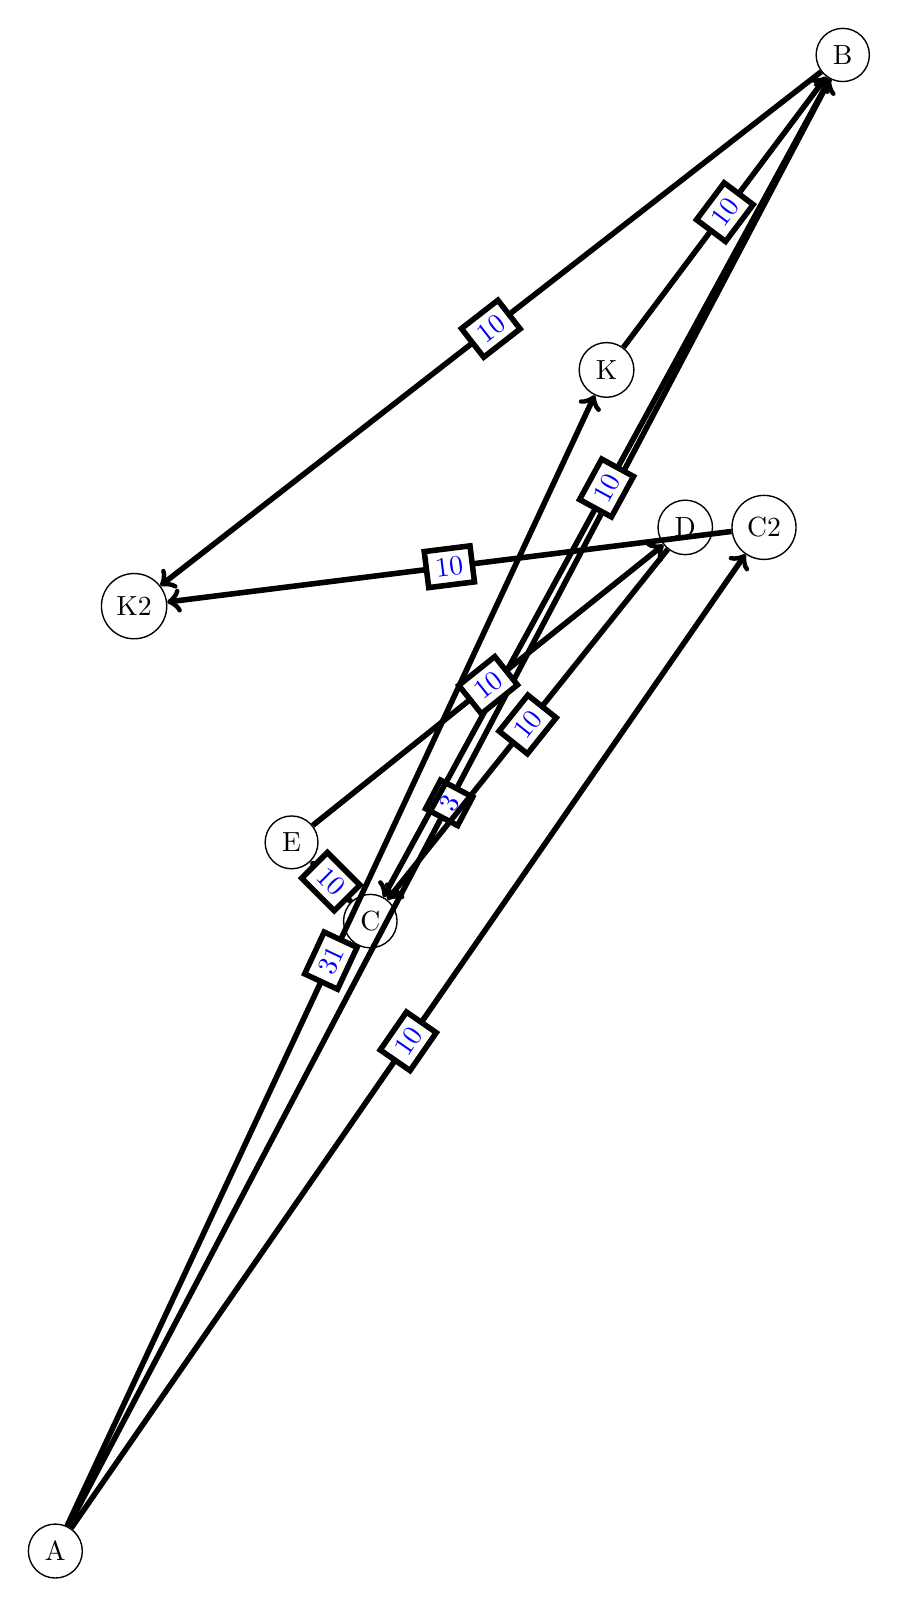
\begin{tikzpicture}

\SetVertexNormal[Shape      = circle,
                 FillColor  = orange,
                 LineWidth  = 2pt]

\SetUpEdge[lw         = 2pt,
            color      = black,
            labelcolor = white,
           labeltext  = red,
           labelstyle = {sloped,draw,text=blue}]


  \GraphInit[vstyle=Normal] 
  \SetGraphUnit{10}
  \tikzset{VertexStyle/.append  style={fill}}

%%% 6 --> 2x3 (divisors)   7 (8)--> 2x4 

   \Vertex[x=0 ,y=0]{A}
   \Vertex[x=10 ,y=19]{B}
   \Vertex[x=4,y=8]{C}
   \Vertex[x=9,y=13]{C2}

   \Vertex[x=8 ,y=13]{D}
   \Vertex[x=3 ,y=9]{E}
   \Vertex[x=7 ,y=15]{K}
   \Vertex[x=1 ,y=12]{K2}
   
  \tikzset{EdgeStyle/.style={->}}

  \Edge[label=$3$](A)(B)
  \Edge[label=$31$](A)(K)
  \Edge[label=$10$](B)(C)
  \Edge[label=$10$](C)(E)
  \Edge[label=$10$](K)(B)
  \Edge[label=$10$](E)(D)
  \Edge[label=$10$](D)(C)
  \Edge[label=$10$](A)(C2)
  \Edge[label=$10$](C2)(K2)
  \Edge[label=$10$](B)(K2)
  

\end{tikzpicture}
\end{center}
\end{document}


